%!TEX root = ../main.tex

\section{Method}
\label{s:method}
% \todo[inline]{Global idea of PN triangles, lit less global than in introduction}
The main goal of point-normal triangles is to improve the visual quality of rendered models, especially on resource-limited hardware environments where e.g. no information about neighboring triangles can be accumulated. We ask the reader to have a look at \cref{fig:preamble:teaser}, with the following question in mind: Which rendering do you prefer? The center and right images both show a rendering using the phong shading and illumination model. The only difference being, that the right image is rendered using poit-normal triangles, with an inner and outer tessellation level of $12.0$. The influence of the tessellation levels is discussed in \crefs{s:implementation}. \citeauthor{vlachos2001curved} formulated the goal of point-normal triangles as: ``soften triangle creases and improve the visual appeal by generating smoother silhouettes and better shading''. \citeauthor{vlachos2001curved} mention, besides the visual improvements, the following benefits of using PN triangles:

\begin{enumerate}[label=(\roman*)]
 	\item 
 		Point-normal triangle construction is \textit{compatible} with the existing graphics API data structures, i.e., vertex arrays together with triangle index streams, where the triangles arrive in unpredictable order.
 	\item 
 		The models are \textit{backward compatible} with hardware that does not support point-normal triangles, with minimal or no changes needed to existing models.
 	\item 
 		No setup of the application, API, or hardware driver is needed. Specifically, hardware is not required to provide random access to neighboring primitives. Consequently the only possible communicated information between primitives are provided by using shared normals at the vertices. This does restrict the models to be rendered somewhat, as discussed in \crefs{sss:method:geometric:properties}.
 	\item 
 		Point-normal triangles are applicable to meshes with \textit{arbitrary topology}.
 	\item 
 		PN-triangle rendering is \textit{fast} and done via \textit{simple implementation} in hardware on the CPU in 2001. At the time of writing point-normal triangles can be rendered via programmable tessellation shaders on the GPU.
 \end{enumerate} 

In the remaining part of this section we discuss the construction of point-normal triangles conceptually as well as mathematically. As mentioned in the introduction, a PN triangle is split in two different components: we refer to \crefs{ss:geometric_component} for a discussion on the geometric component and to \crefs{ss:normal_component} for the review of the normal component.

\begin{figure}
	\centering
	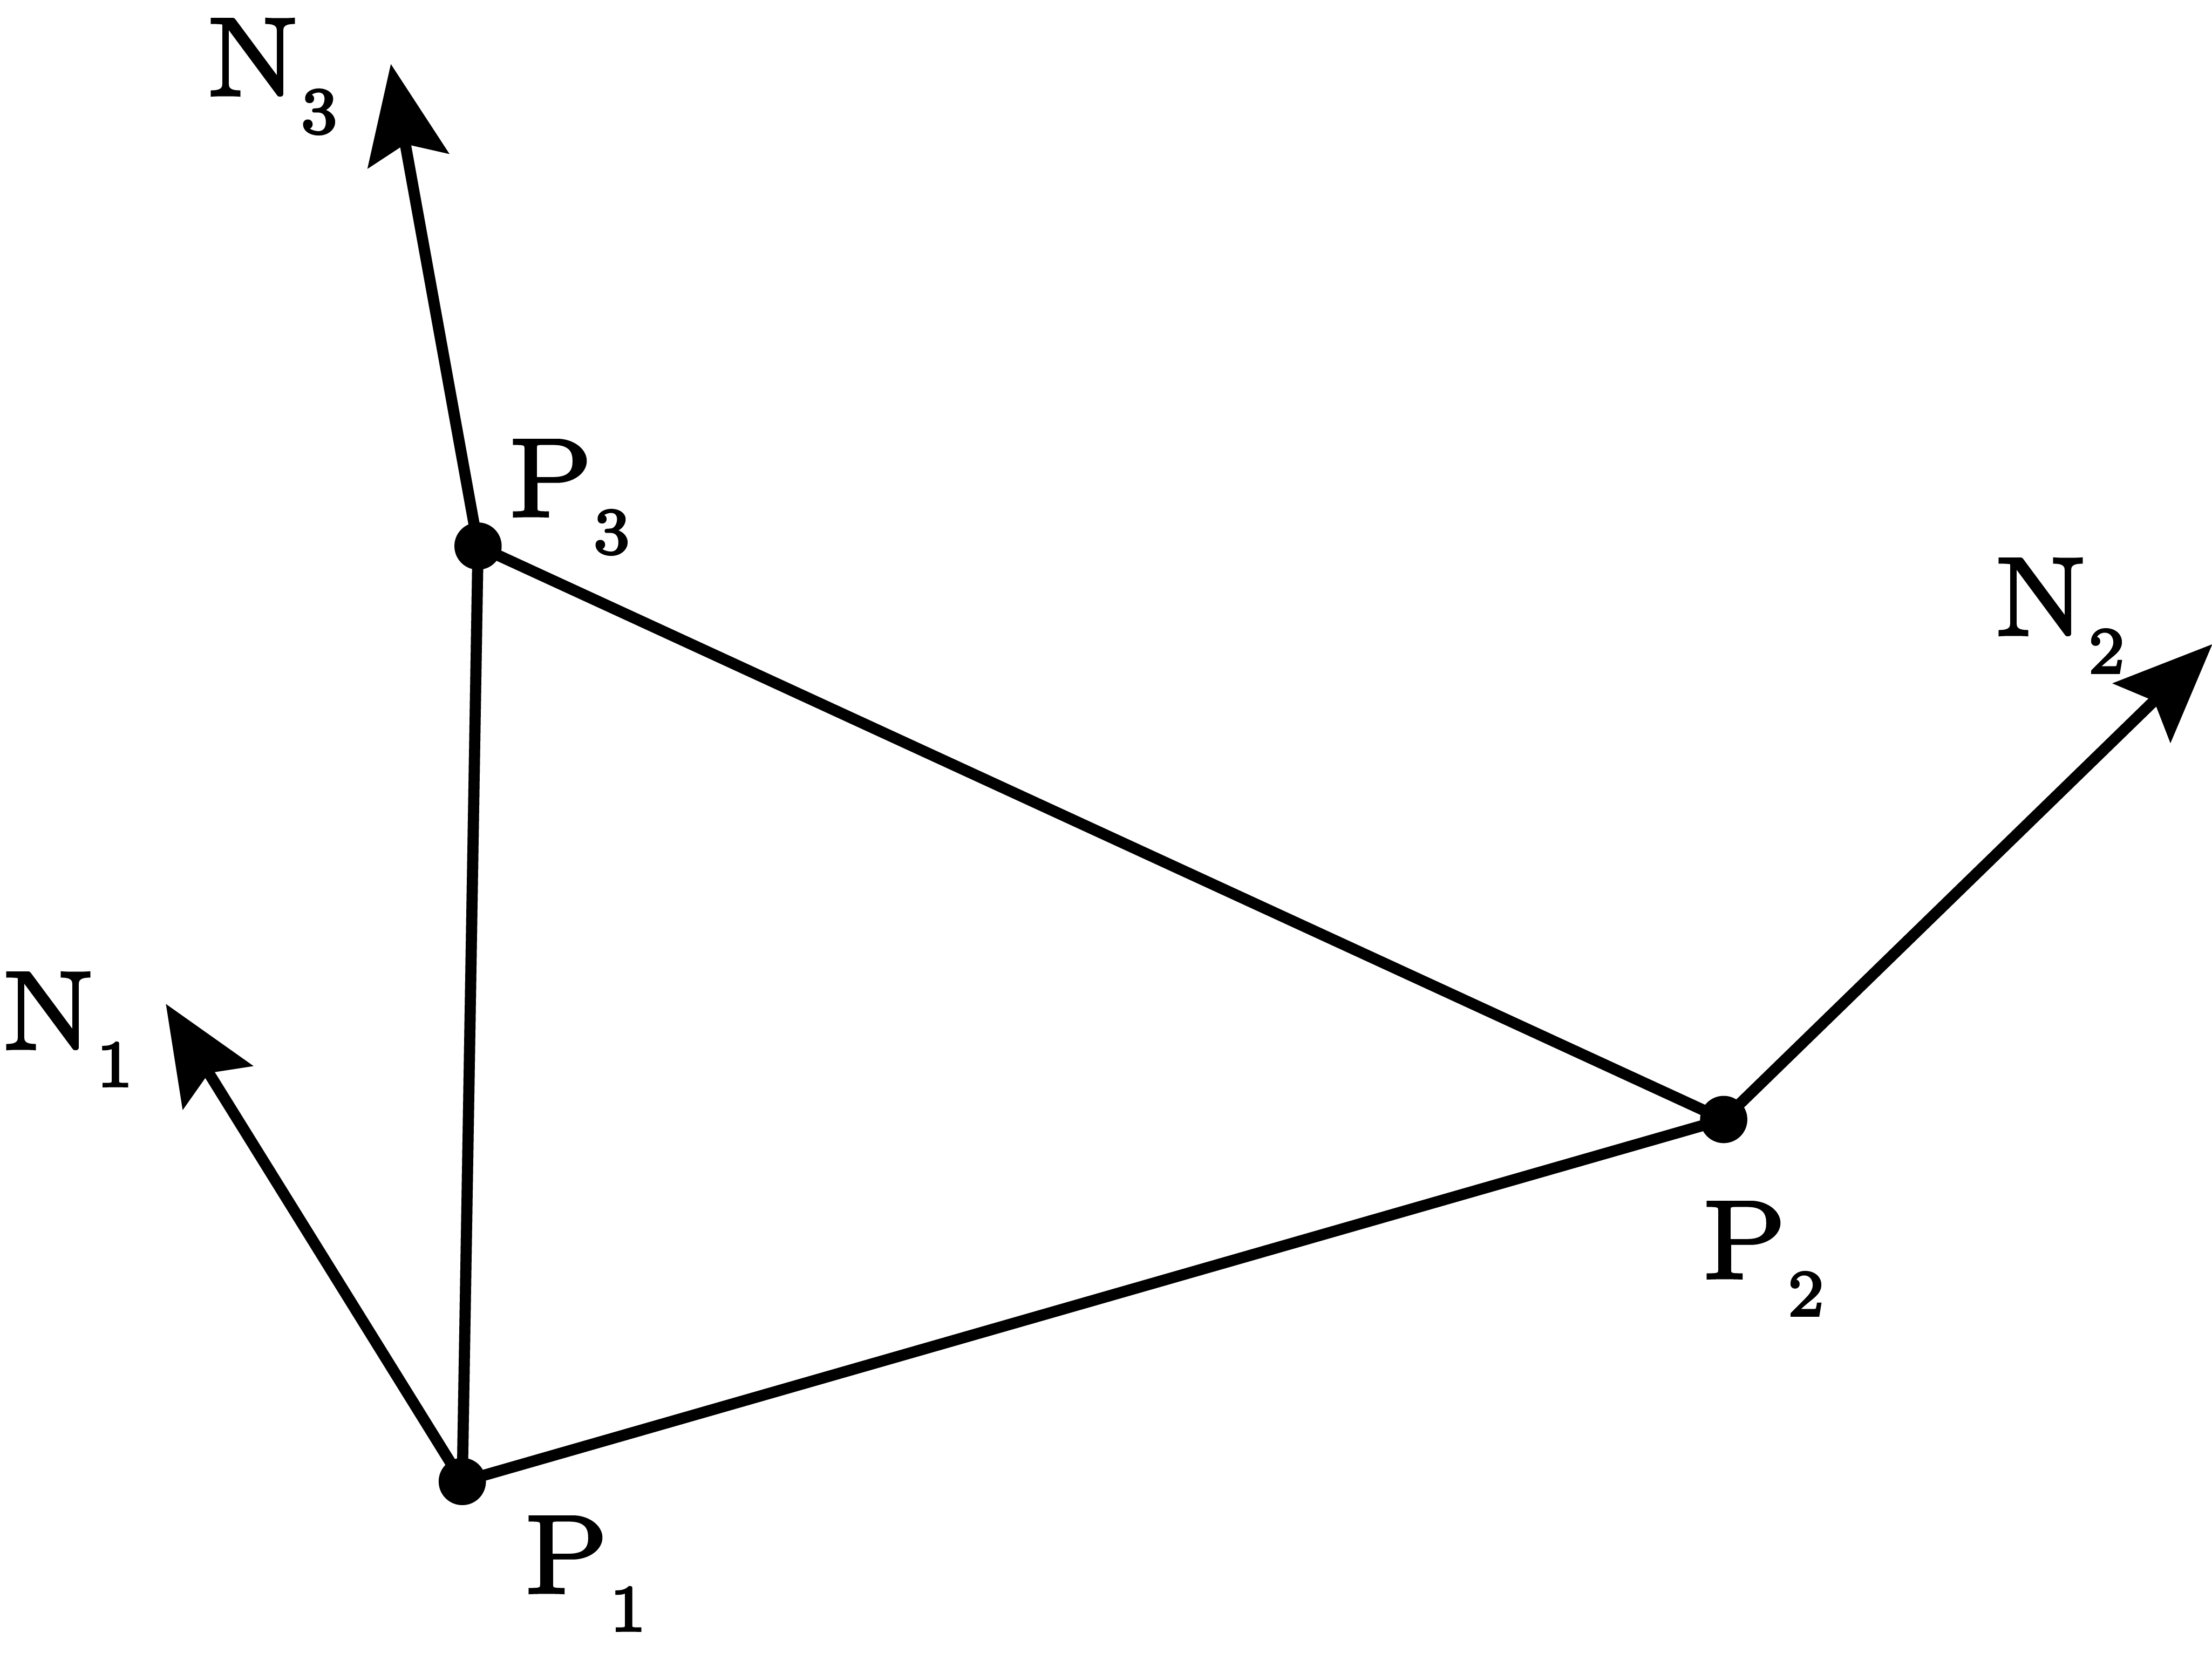
\includegraphics[width=0.4\textwidth]{./content/img/method/inputPrimitive.png}
	\caption{An input primitive based on which a point-normal triangle can be computed. The input primitive consists of three vertices, $P_1$, $P_2$ and $P_3$, and three vertex normals, $N_1$, $N_2$, $N_3$. Note that only the information of a single primitive is used during the construction of both the geometric and the normal component, i.e. no information about neighboring primitives is used.}
	\label{fig:method:input_primitive}
\end{figure}

% %!TEX root = ../main.tex

\subsection{Geometric component}
\label{ss:geometric_component}
Let us emphasize again that the only used information for the construction of the geometric and normal component are the three vertices with associated normals, that define a single primitive. The vertices contain the vertex \textit{xyz}-coordinates together with a unique shared normal per vertex, i.e., the normal of each vertex is the same for every primitive using that vertex. Figure \ref{fig:method:input_primitive} shows an illustration of an input primitive. Each point-normal triangle construction starts with an input primitive of this form.

\begin{figure}
	\centering
	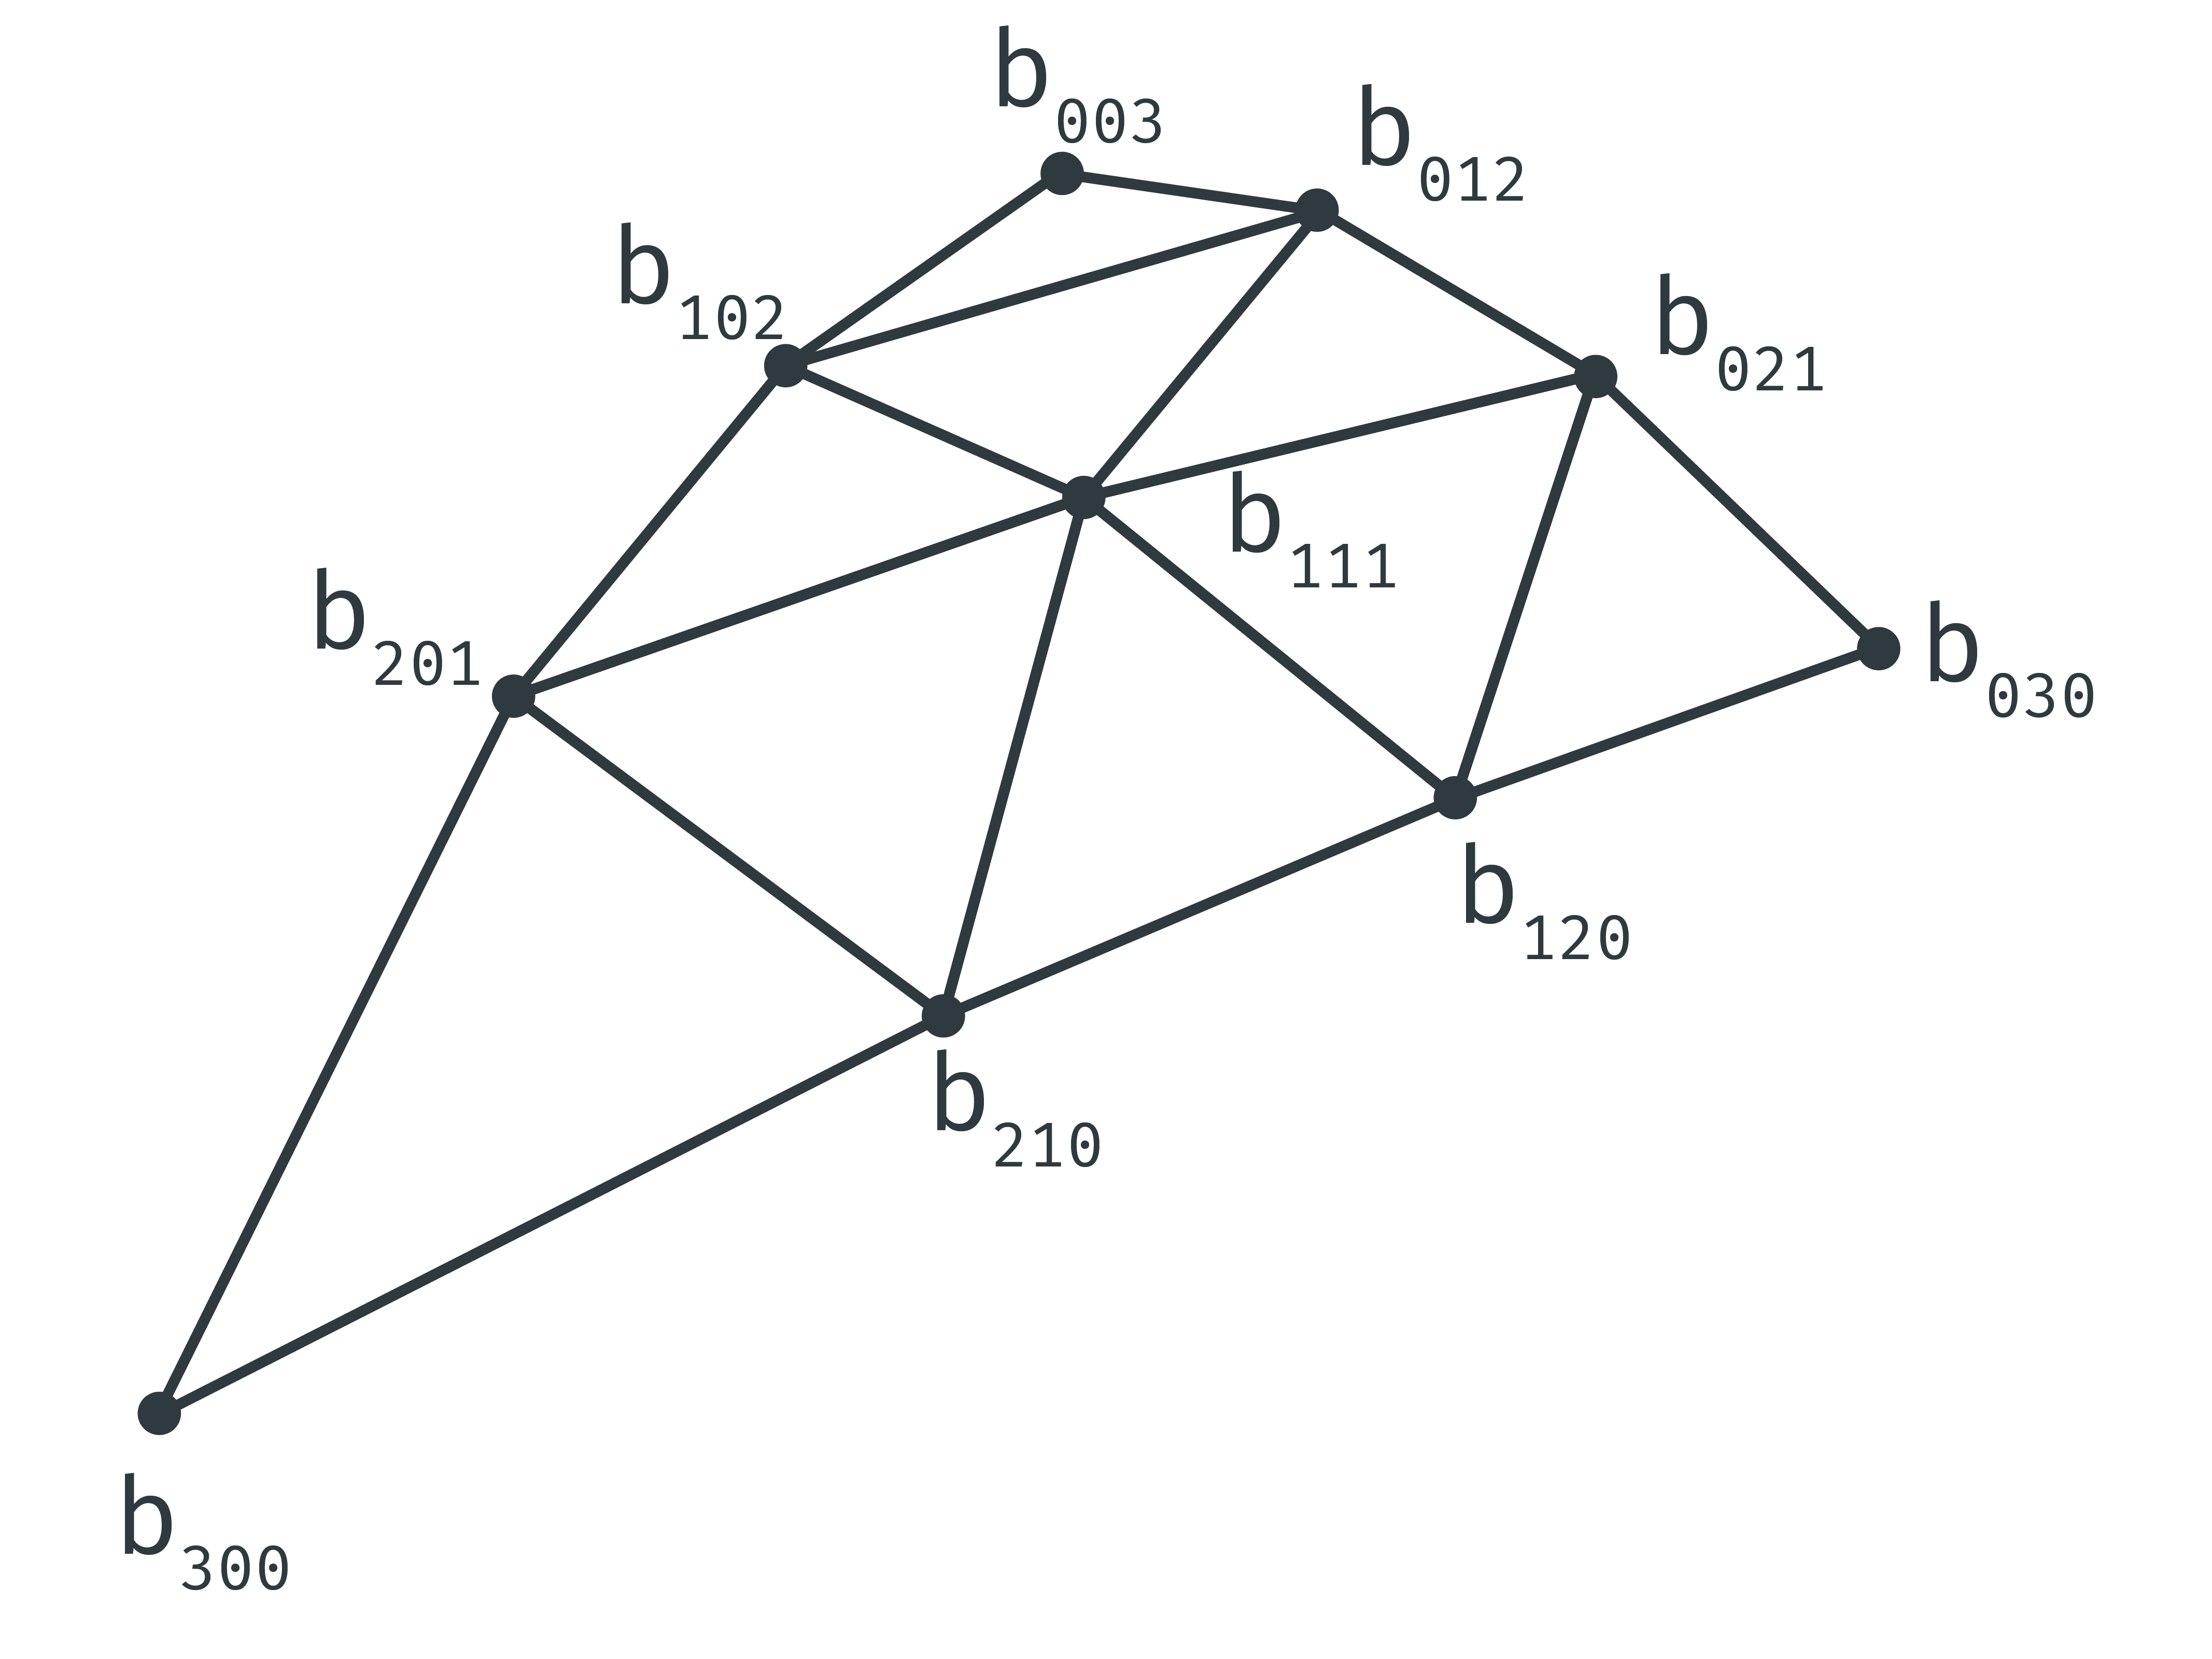
\includegraphics[width=0.45\textwidth]{./content/img/method/geometry.png}
	\caption{The geometric component of a point-normal triangle, i.e. the control net of a cubic Bézier triangle.}
	\label{fig:method:control_net}
\end{figure}
%
% ## Geometric component defined by triangluar cubic Bezier patch.
%
In the next subsection we discuss the definition of the geometry of a point-normal triangle. In subsection \crefs{sss:control_point_construction} we discuss the construction of the control points that define the geometry. 

\subsubsection{Basic form}
The geometric component of a point-normal triangle is defined as a triangular cubic Bézier patch. Such a patch $b(u,v)$ is defined as follows:
%
\begin{align}
\noalign{$b(u,v): \quad R^2 \mapsto R^3,\quad$ for $w = 1 - u - v, \quad u, v, w \geq 0$}
\begin{split}\label{eq:method:cubic_bezier_patch}
    b(u,v) ={}& \sum_{i + j + k = 3} b_{ijk}\frac{3!}{i!j!k!} u^i v^j w^k\\
      	   ={}& b_{300}w^3 + b_{030}u^3 + b_{003}v^3\\
      	    {}& + b_{210}3w^3 + b_{120}3wu^2 + b_{201}3w^2v\\
      	    {}& + b_{021}3u^2v + b_{102}2wv^2 + b_{012}3uv^2\\
      	    {}& + b_{111}6wuv.
\end{split}
\end{align}
%
The $b_{ijk}$ parameters in equation \ref{eq:method:cubic_bezier_patch} are the control points of the patch, also called coefficients. In \cref{fig:method:control_net} the visualization of the network of these control points is shown. We group the coefficients in three different groups, as their construction differs:
%
\begin{align*}
	\text{vertex coefficients: } {}&  b_{300},\ b_{030},\ b_{003} \\
	\text{tangent coefficients: } {}&  b_{210},\ b_{120},\ b_{021},\ b_{012},\ b_{102},\ b_{201}\\
	\text{center coefficient: }   {}&  b_{111}\\
\end{align*}

The formula in \eqref{eq:method:cubic_bezier_patch} can be used to evaluate any point parameterized by the barycentric coordinates $(u,v,w)$, on the patch. This is used in the sub-triangulation stage of the rendering process. In this stage the cubic Bézier surface is approximated by using a number of smaller flat triangles; these flat triangles are the triangles that are actually rendered. The number of sub-triangles is determined by the level of detail (lod). For the original sub-triangulation we refer the reader to \textcite{vlachos2001curved}, as this is where the implementation presented here deviates from the original. Details about this are provided in \crefs{s:implementation}.

As stated above the definition of the geometry of a point-normal triangle is a cubic Bézier patch. This degree of patches is a trade-off between simplicity, visual performance, and computational cost. Quadratic patches do not provide the same modeling range of a surface as a cubic patch, \citeauthor{boubekeur2008phong} \cite{boubekeur2008phong}. For example, a cubic representation is necessary to capture inflections implied by the triangle position and normal data. \citeauthor{vlachos2001curved} state that there is no additional data to suggest a higher degree is needed, and that therefore they settled on the form of $b(u,v)$ as presented in \crefe{eq:method:cubic_bezier_patch}.

\subsubsection{Coefficients} \label{sss:control_point_construction}
This section discusses how the `curved' control net geometry, (see \cref{fig:method:control_net}) is calculated from the flat input primitive shown in \cref{fig:method:input_primitive}. The input primitive provides the positions $P_1, P_2, P_3 \in \Real^3$ and normals $N_1, N_2, N_3 \in \Real^3$. The coefficients $b_{ijk}$ are computed as follows:
%
\begin{enumerate}[label=(\roman*)]
	\item 
		Initially, the coefficients $b_{ijk}$ are spread uniformly, i.e., the intermediate position of $b_{ijk}$ is calculated using the formula $(i P_i + j P_2 + kP_3) / 3$. 
	\item 
		The intermediate positions of the vertex coefficients are the same as their final positions, see equation \eqref{eq:method:vertex_coefficients}. Their intermediate position places them at the vertices of the input triangle, and this is where they are required to stay to keep the mesh watertight.
	\item 
		The tangent coefficients are placed at their final position by projecting the intermediate position into the tangent plane of the closest corner, see equation \eqref{eq:method:tangent_coefficients}. This is illustrated in \cref{fig:method:geometry_tangent_projection.png}.
	\item The center coefficient is moved to the average of the tangent coefficients plus $1/2$ times the distance it had to travel from its intermediate position, see equation \eqref{eq:method:center_coefficient}.
\end{enumerate}
%
\begin{figure}
	\centering
	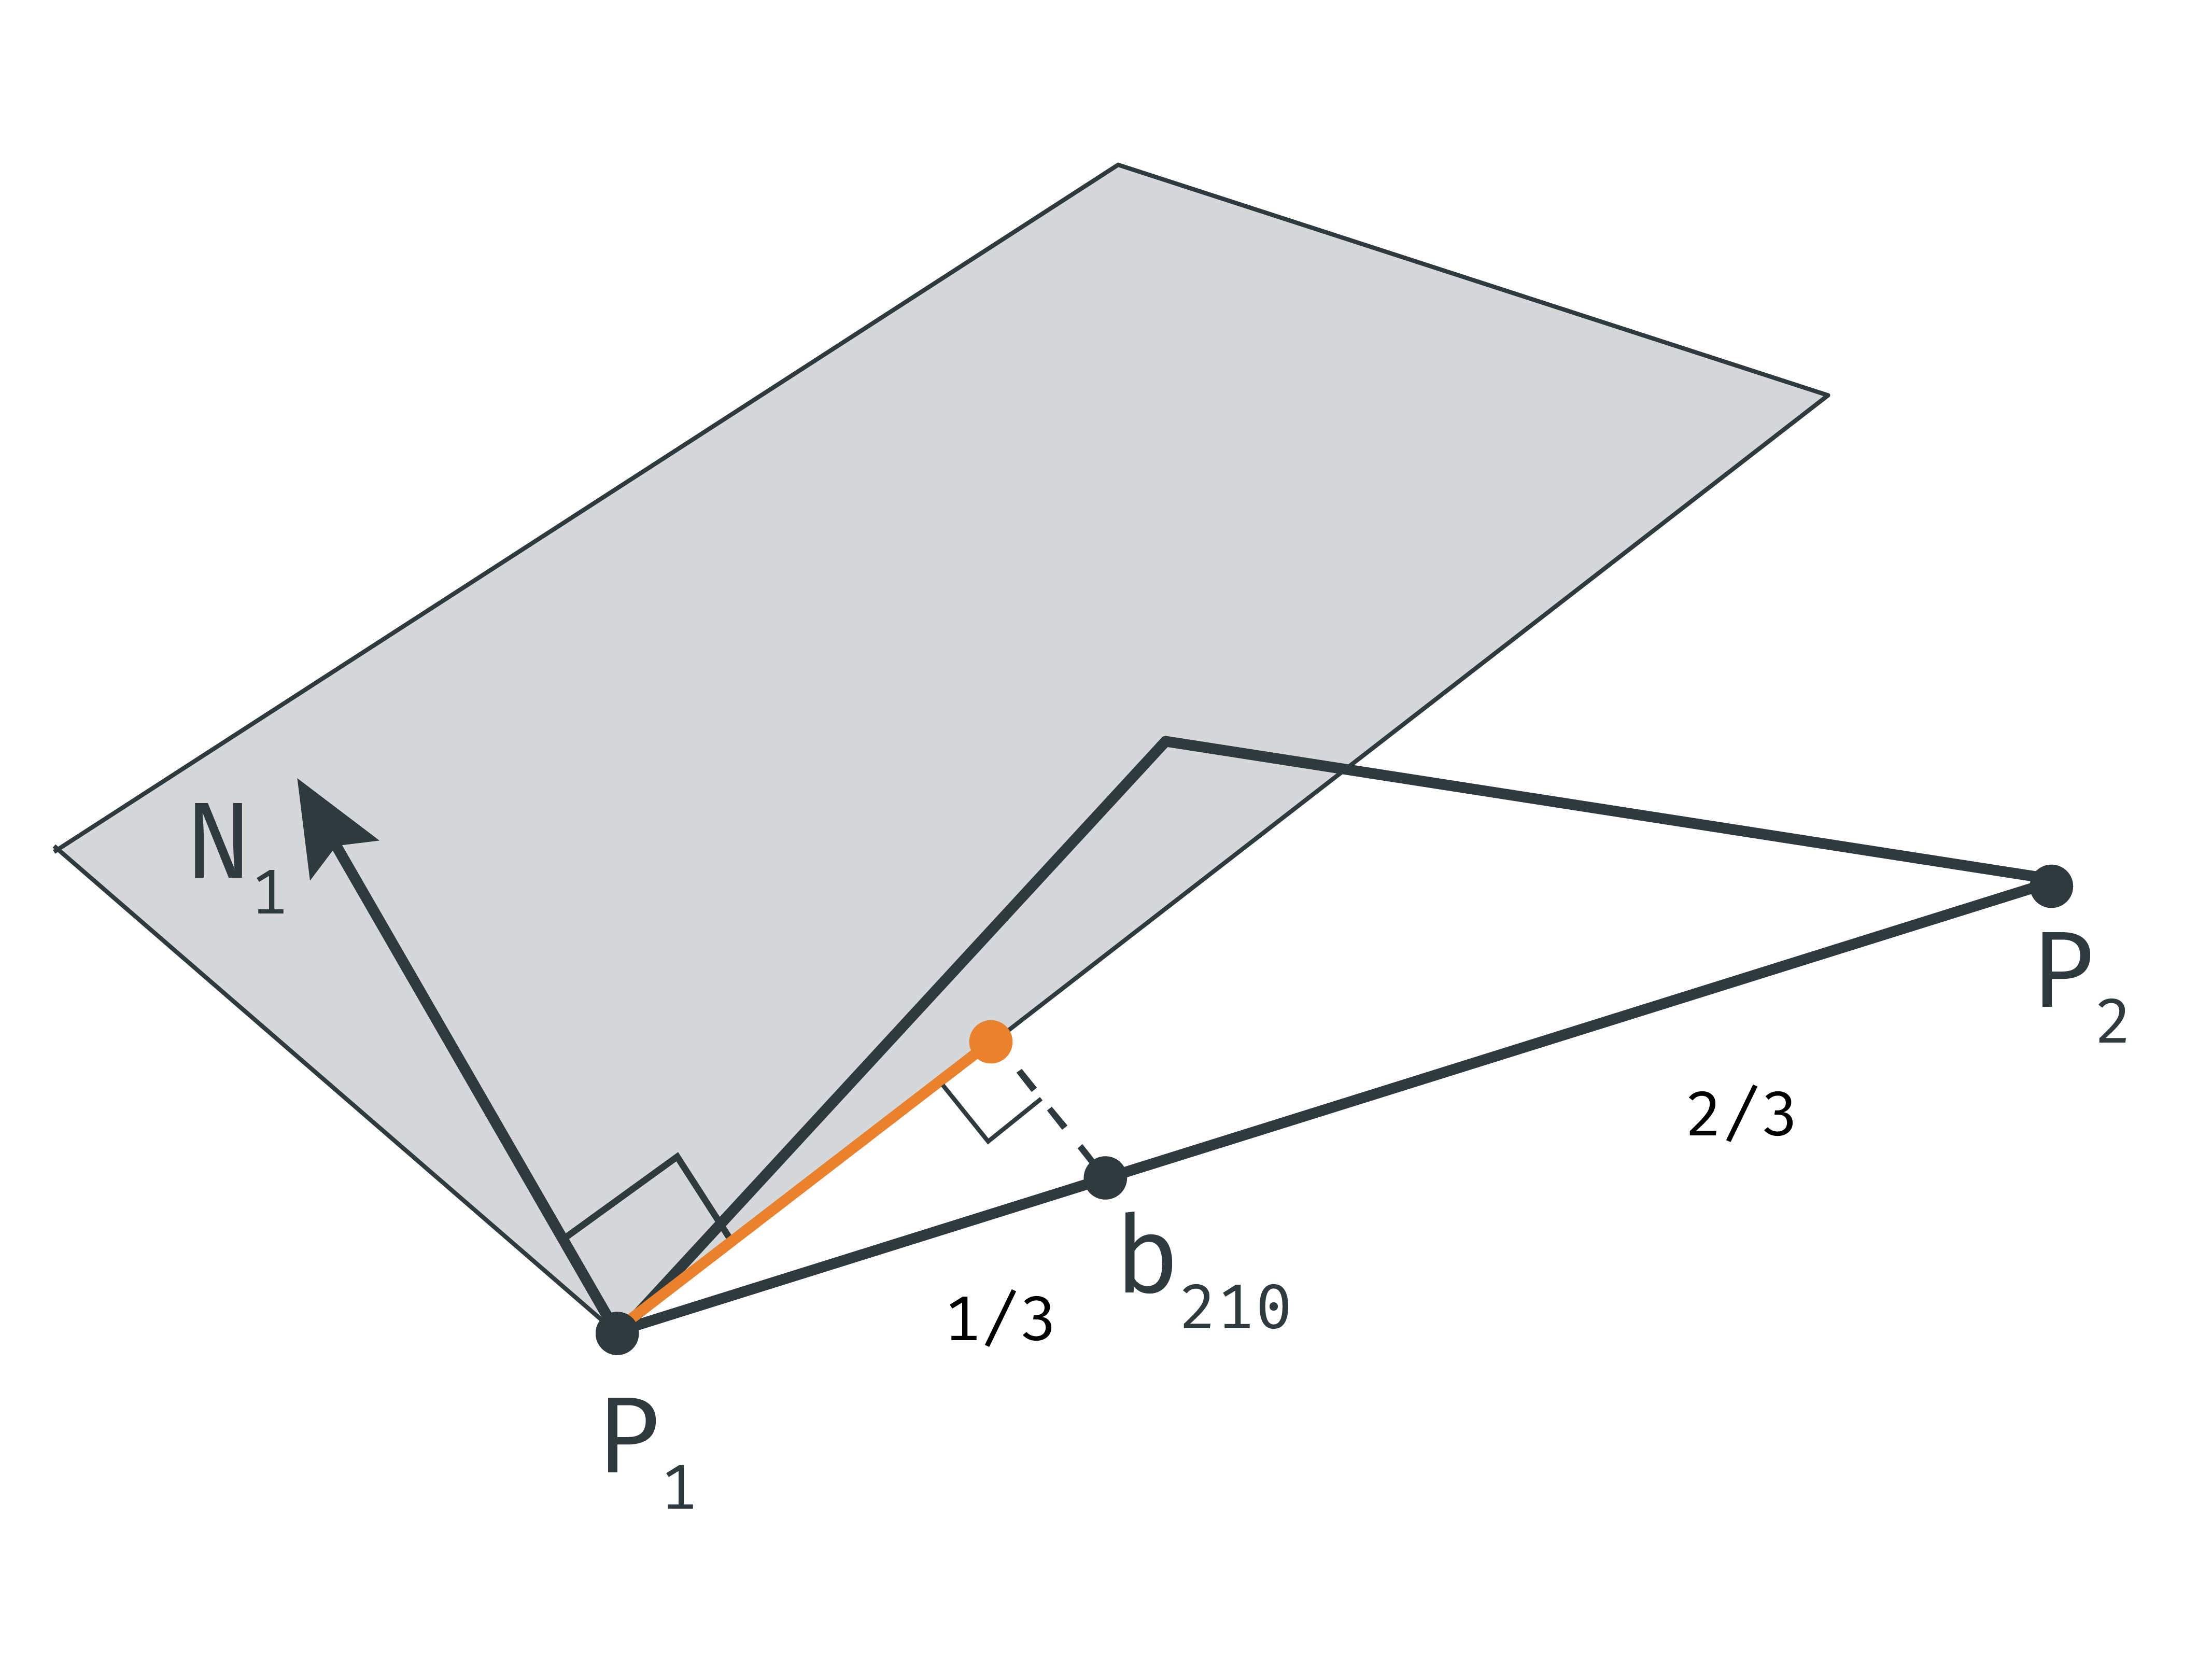
\includegraphics[width=0.45\textwidth]{./content/img/method/geometry_tangent_projection.png}
	\caption{Projection of a tangent coefficient $b_{210}$ to the tangent plane of the closes corner $P_1$.}
	\label{fig:method:geometry_tangent_projection.png}
\end{figure}


The following set of formulas describe how the positions of the coefficients are calculated. For clarity, we group together the formulas in the same way as the coefficients. This gives the following formulas for the \textit{vertex coefficients}:
\begin{align}\label{eq:method:vertex_coefficients}
	b_{300} = P_1,\ b_{030} = P_2,\ b_{003} = P_3.
\end{align}

The tangent coefficients are given by the projection of a point $Q$ onto the plane defined by the normal $N$ of the point $P$. The projected point $Q'$ is then given by: $Q' = Q - wN$, where $w = (Q - P) \cdot N$. Using this, the following set of formulas give the positions of the \textit{tangent coefficients}:
\begin{align}\label{eq:method:tangent_coefficients}
	w_{ij} = {}& (P_j - P_i) \cdot N_i \in \Real \nonumber\\
	b_{210} = {}& (2 P_1 + P_2 - w_{12}N_1) / 3,\nonumber\\
	b_{120} = {}& (2 P_2 + P_1 - w_{21}N_2) / 3,\nonumber\\
	b_{021} = {}& (2 P_2 + P_3 - w_{23}N_2) / 3, \\
	b_{012} = {}& (2 P_3 + P_2 - w_{32}N_3) / 3,\nonumber\\
	b_{102} = {}& (2 P_3 + P_1 - w_{31}N_3) / 3,\nonumber\\
	b_{201} = {}& (2 P_1 + P_3 - w_{13}N_1) / 3. \nonumber
\end{align}

The last coefficient is the center coefficient which is, as stated before, moved to the average of the previous computed tangent coefficients plus $1/2$ times the distance it traveled from its intermediate location to that average position. The \textit{center coefficient}, is computed by:
\begin{align}\label{eq:method:center_coefficient}
	E = {}& (b_{210} + b_{120} + b_{021} \nonumber \\
		{}& + b_{012} + b_{102} + b_{201}) / 6, \nonumber\\
	V = {}& (P_1 + P_2 + P_3) / 3, \\
	b_{111} = {}& E + (E - V) / 2. \nonumber
\end{align}
Combining \eqref{eq:method:vertex_coefficients} through \eqref{eq:method:center_coefficient} transforms the input primitive (see \cref{fig:method:input_primitive}) to the control net shown in \cref{fig:method:control_net}.


\subsubsection{Properties}
\label{sss:method:geometric:properties}
\citeauthor{vlachos2001curved} have shown that point-normal triangles do not deviate too much from the original triangle. This is an important property since this ensures that the shape of the model is preserved and adjacent triangles do not interfere with each other. 

By demanding shared normals, i.e., one unique normal per vertex, the boundary between two point-normal triangles is generated by the same algorithm, thus the surface is water tight. Except at the corners, PN triangles do not usually join with tangent continuity \cite{vlachos2001curved}. \Cref{fig:method:cracks} illustrates what happens if normals are not shared.

\begin{figure}
	\ooit{Moeten dit plaatje eigenlijk maken met driehoeken.}
	\centering
	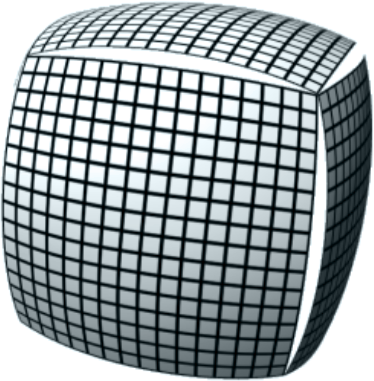
\includegraphics[width=0.4\columnwidth]{./content/img/method/cracks.png}
	\caption{Illustration of what would happen if one renders a model using point-normal triangles where vertices have different normals, depending on the associated faces. Image taken from \cite{mcdonald2010crack}.}
	\label{fig:method:cracks}
\end{figure}

%!TEX root = ../main.tex

\subsection{Normal component}\label{ss:normal_component}
% What?
This section discusses the parametrization of both the `fake' and `real' normals. We differentiate between these two normal types because originally point-normal triangles normals are interpolated based on a quadratic patch, the `fake' normals (see \crefs{sss:method:normals:fakeNormals}), whereas one would get the `real' normals by calculating them based on the actual surface (see \crefs{sss:method:normals:realNormals}).

It should be noted that, just as with the geometric component, the normal component of the point-normal triangle is computed solely based on the input primitive, i.e., the vertex positions and their normals, as shown in \cref{fig:method:input_primitive}. 

\begin{figure}
	\centering
	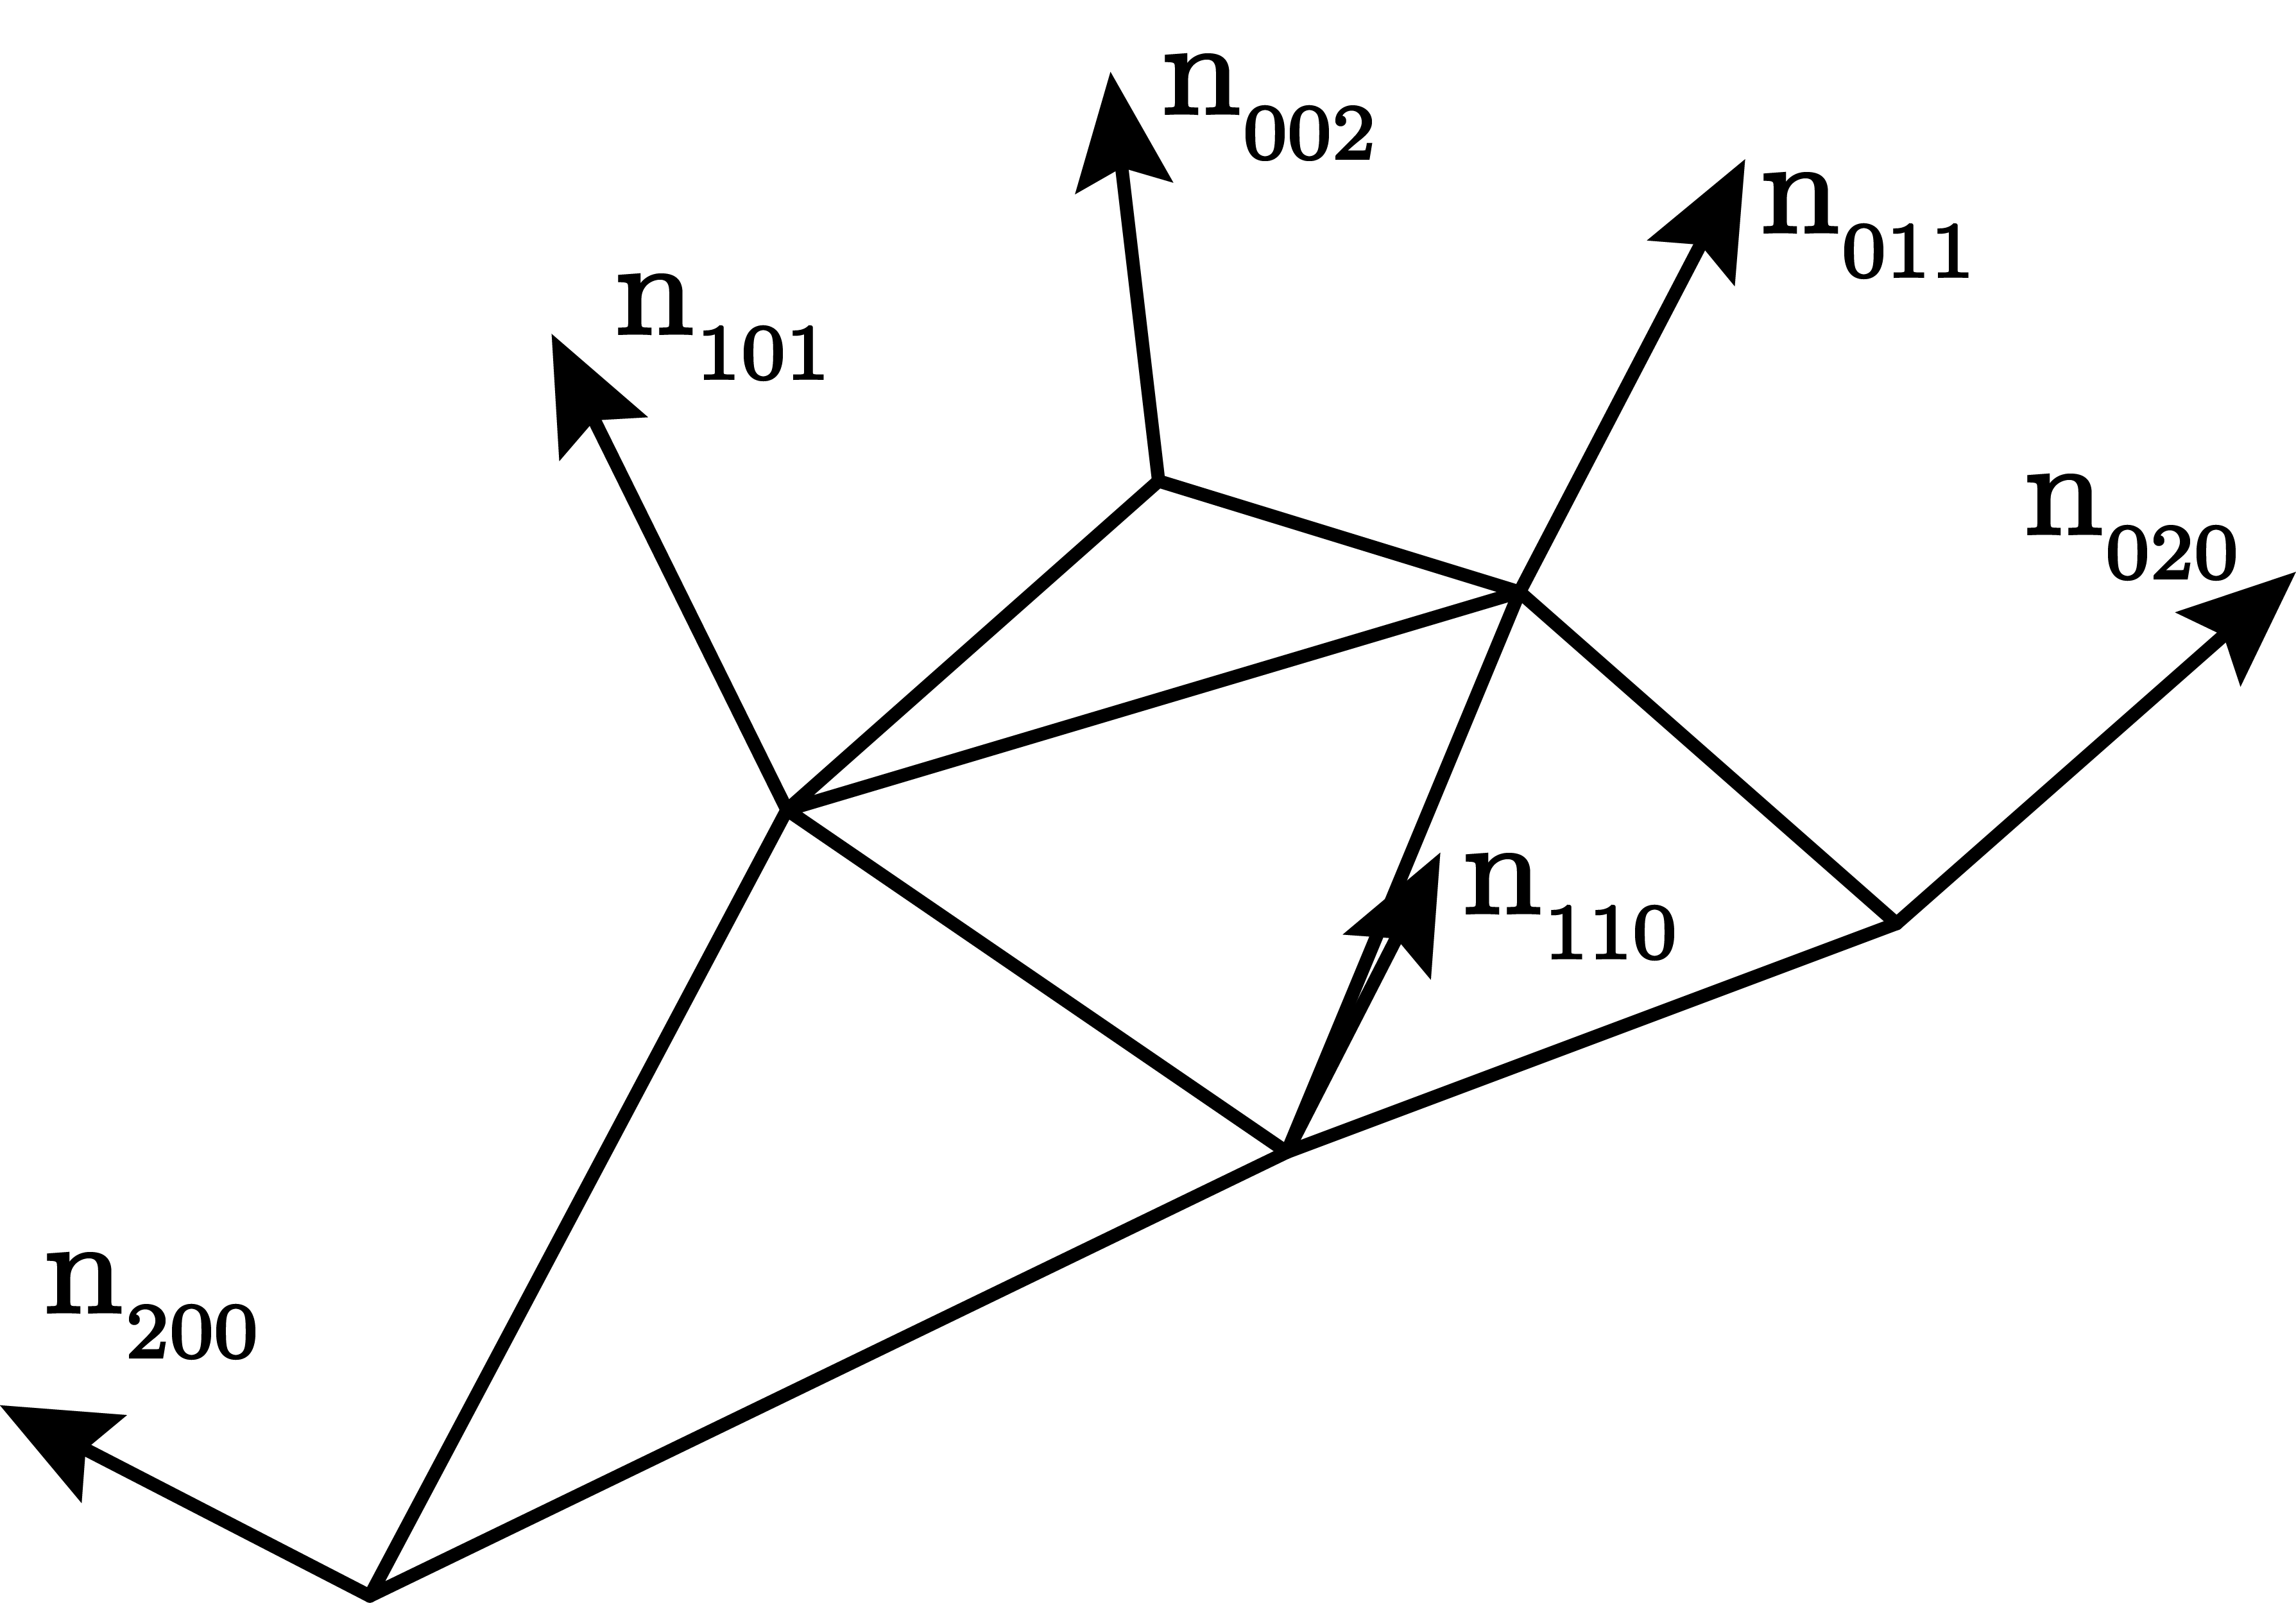
\includegraphics[width=0.45\textwidth]{./content/img/method/normals.png}
	\caption{The normal field of the point-normal triangle.}
	\label{fig:method:normal_field}
\end{figure}

\subsubsection{Fake normals}
\label{sss:method:normals:fakeNormals}
	\citeauthor{vlachos2001curved} define the `fake' normals using a quadratic function $n(u,v)$:
	\begin{align}
	\noalign{$n(u,v): \quad R^2 \mapsto R^3,\quad$ for $w = 1 - u - v, \quad u, v, w \geq 0$}
	\begin{split}\label{eq:method:quadratic_normal_patch}
	    n(u,v) ={}& \sum_{i + j + k = 2} n_{ijk}u^i v^j w^k,\\
	      	   ={}& n_{200}w^2 + n_{020}u^2 + n_{002}v^2\\
	      	    {}& + n_{110}wu + n_{011}uv + n_{101}wv\\
	\end{split}
	\end{align}
	The coefficients of this quadratic `patch' are the normals shown in \cref{fig:method:normal_field}. The normals are computed for a point, halfway on every edge, i.e., $(u,v,w) = (\frac{1}{2}, \frac{1}{2}, 0)$, $(0, \frac{1}{2}, \frac{1}{2})$, $(\frac{1}{2}, 0, \frac{1}{2})$. Point-normal triangles use quadratically varying normals to be able to capture the inflection points that are possible due to the cubic geometric component. 

	\Cref{fig:method:linear_vs_quadratically_varying} illustrates why one needs quadratic patches to capture these inflection points. \Cref{fig:method:linear_vs_quadratically_varying} illustrates two cases: \cref{fig:method:normal:both} shows that when the normals point in a different direction the surface will be parabolic, and no inflection point exists. In this case both linear and quadratically varying normals are able to capture the surface. In \cref{fig:method:normal:linear} and \cref{fig:method:normal:quadratic} the case were an inflection point exists is shown. We see that (\cref{fig:method:normal:linear}) linear varying normals do not capture the inflection point, i.e., give incorrect normals. The quadratically varying normals do give the correct normals (\cref{fig:method:normal:quadratic}), i.e, they capture the inflection point.

	\begin{figure}
		\centering
		\begin{subfigure}{\columnwidth}
			\centering
			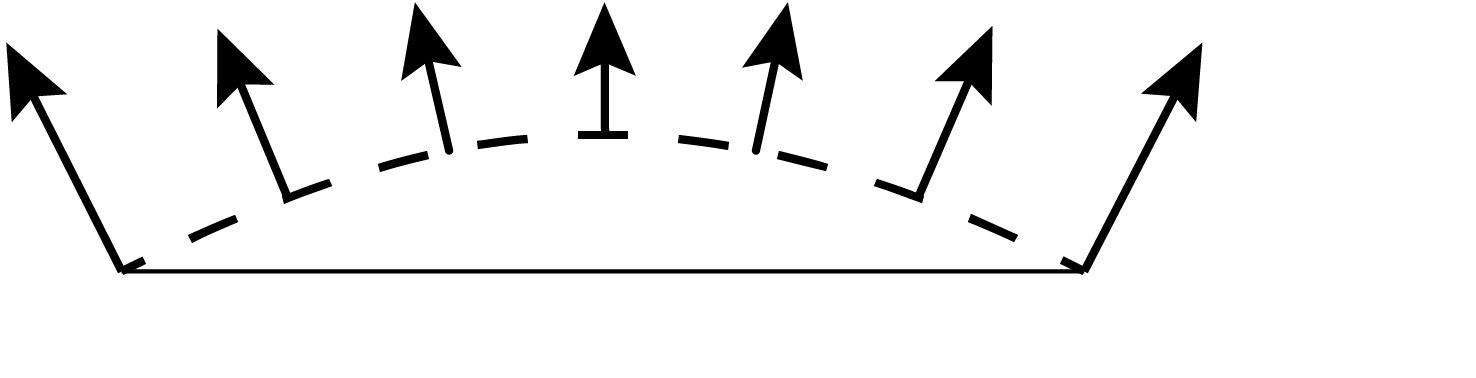
\includegraphics[width=0.8\textwidth]{./content/img/method/linearVsQuadraticNormals_both.png}
			\caption{Vector averaging with either linear or quadratic over a curve without inflections.}
			\label{fig:method:normal:both}
		\end{subfigure}
		\begin{subfigure}{\columnwidth}
			\centering
			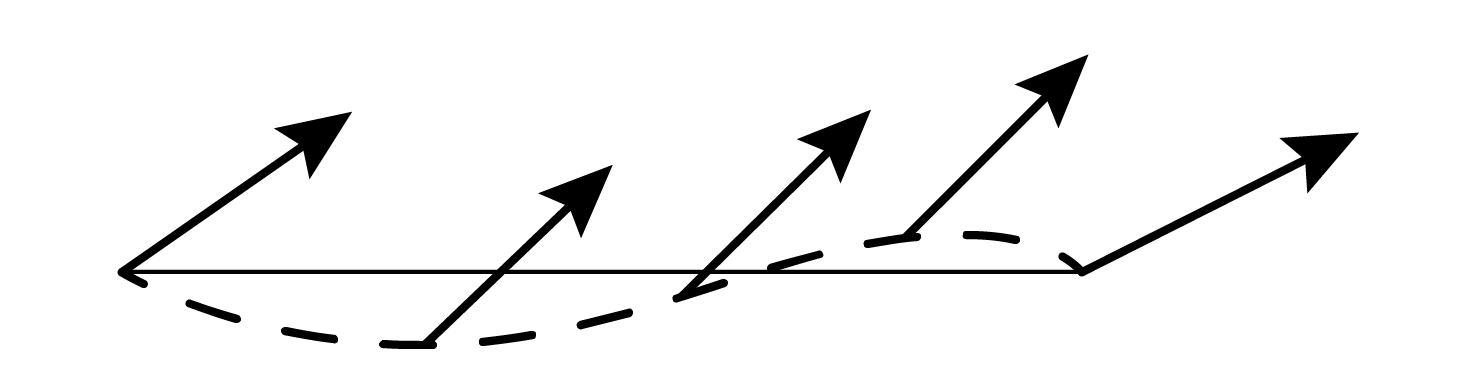
\includegraphics[width=0.8\textwidth]{./content/img/method/linearVsQuadraticNormals_linear}
			\caption{Vector averaging with linear interpolation over a curve with an inflection.}
			\label{fig:method:normal:linear}
		\end{subfigure}	
		\begin{subfigure}{\columnwidth}
			\centering
			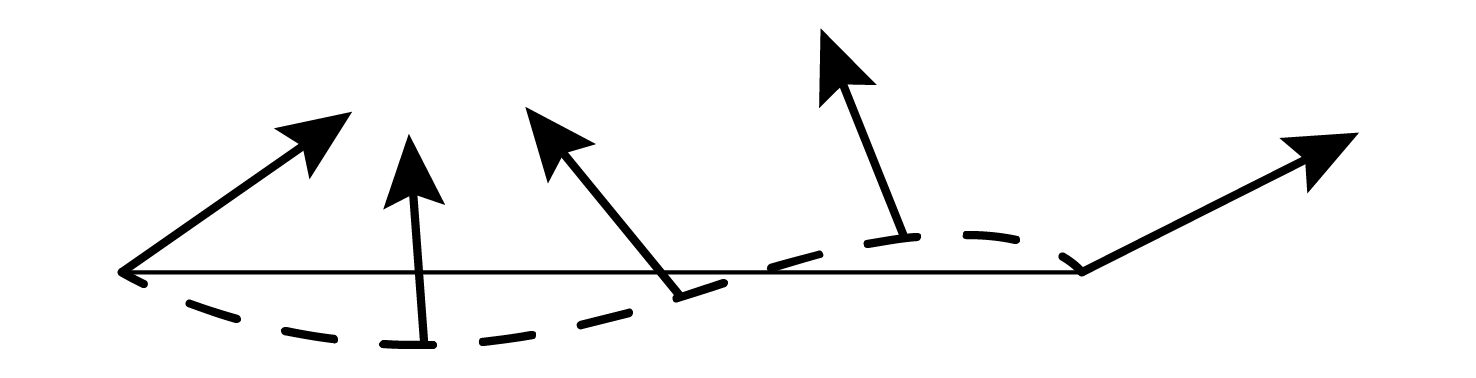
\includegraphics[width=0.8\textwidth]{./content/img/method/linearVsQuadraticNormals_quadratic}
			\caption{Vector averaging with quadratic interpolation over a curve with an inflection.}
			\label{fig:method:normal:quadratic}
		\end{subfigure}			
		\caption{Examples of normal vector averaging over an edge. The dashed lines indicate the profile of the surface that should be approximated. The normals of a curves without inflections are correctly approximated by both linear and quadratic interpolation, see \cref{fig:method:normal:both}. The normals of a curve with inflections are incorrectly approximated with \subref{fig:method:normal:linear} linear interpolation and correctly with \subref{fig:method:normal:quadratic} interpolation. Image \subref{fig:method:normal:both} was adapted from \cite{van1997phong}, image \subref{fig:method:normal:linear} and \subref{fig:method:normal:quadratic} from \cite{vlachos2001curved}.}
		\label{fig:method:linear_vs_quadratically_varying}
	\end{figure}

	\todo[inline]{Discuss parametrization of `quadratic' patch}

	Using the function $n(u,v)$, see \eqref{eq:method:quadratic_normal_patch}, the normal of any point parametrized by the barycentric coordinates $(u,v)$ can be calculated. To do this we first need to define a control net. We consider two different types of coefficients: the vertex normals, $n_{200}$, $n_{020}$, and $n_{002}$; and the edge normals, $n_{110}$, $n_{011}$, and $n_{101}$.
	\todo[inline]{Discuss the construction of the control points for the `quadratic' patch}

	An edge normal is calculated by taking the average of the two input vertex normals of the vertices of the edge. After this step this looks like the image shown in \cref{fig:method:normal:linear}. To capture the inflection point the average normal is then reflected across the plane perpendicular to the edge, see \cref{fig:method:normal:reflection}. When a inflection point exists this will give the correct mid-edge normal (see \cref{fig:method:normal:quadratic}) and this will also not alter the normal field if no inflection point is present, e.g., imagine reflecting the mid-edge normal of the curve shown in \cref{fig:method:normal:both}, this will result in the same normals.

	\begin{figure}
		\centering
		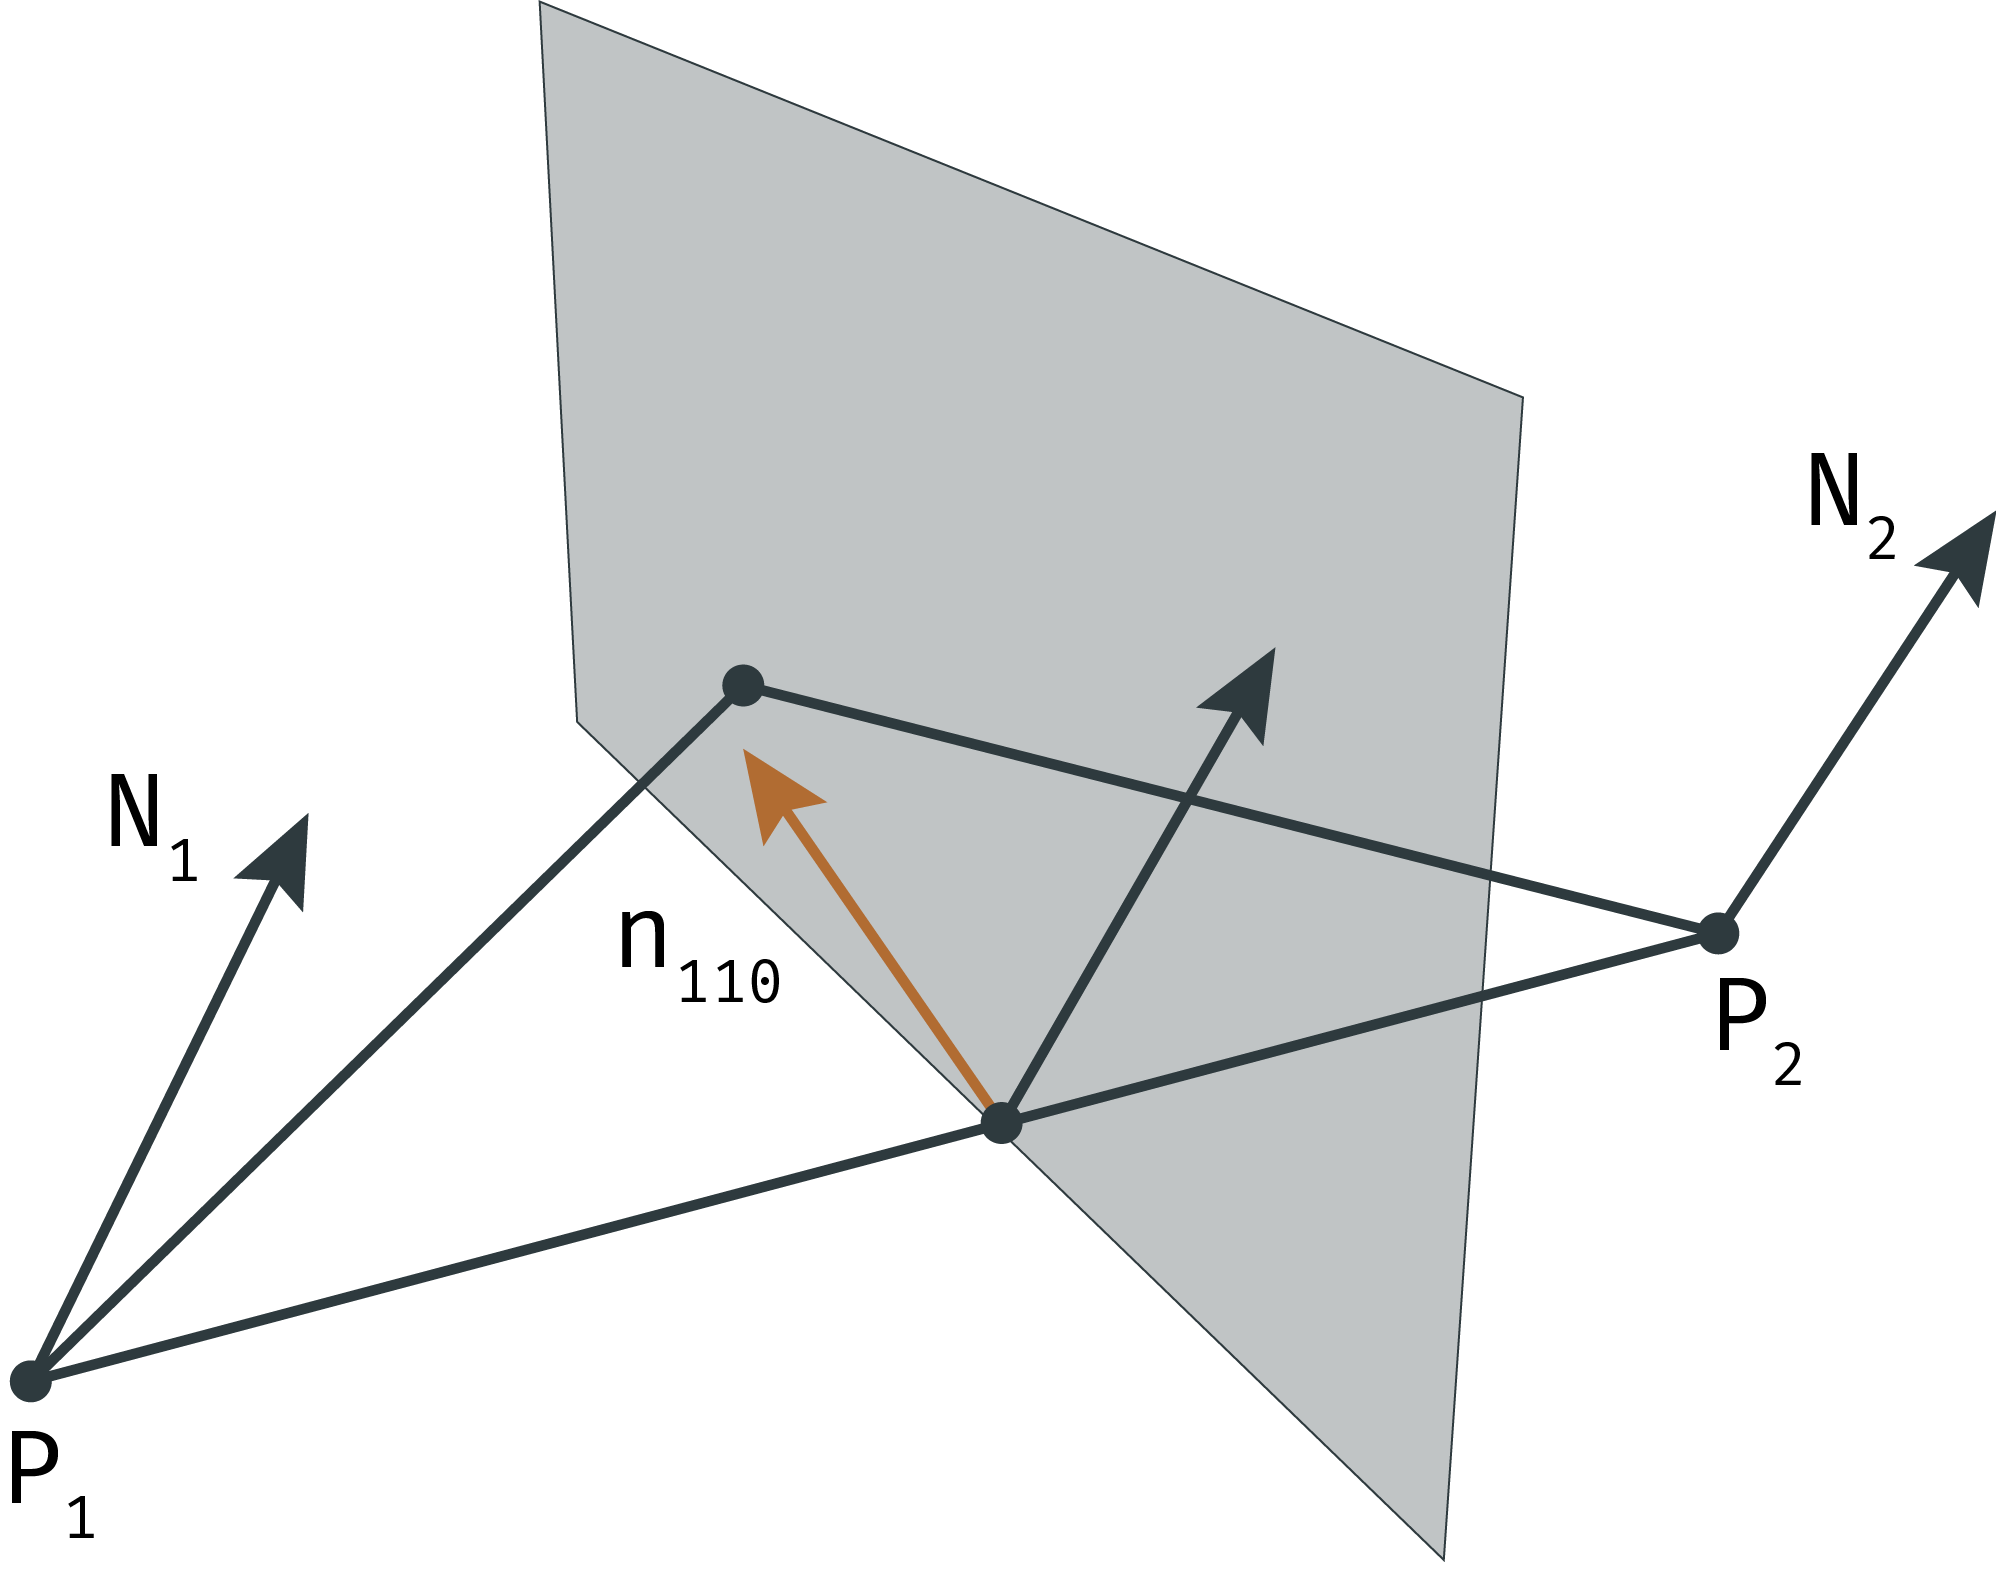
\includegraphics[width=0.45\textwidth]{./content/img/method/normal_reflection.png}
		\caption{Construction of the mid-edge normal coefficient, used for quadratically varying normals. The two input normals are averaged and then reflected reflected across the plane perpendicular to the edge.}
		\label{fig:method:normal:reflection}
	\end{figure}

	The vertex normals are simply the normals provided by the input primitive.

\subsubsection{Real normals}
\label{sss:method:normals:realNormals}
		\todo[inline]{Discuss how to compute the real normals given the geometric component}
		The real normals are computed based on the geometric component of the point-normal triangle. This is done by taking the cross product of the the partial derivatives with respect to $u$ and $v$. For the partial derivatives with respect to $u$ and $v$ see \eqref{eq:method:normal:partialU} and \eqref{eq:method:normal:partialV} respectively.

		\begin{align} \label{eq:method:normal:partialU}
			\frac{\partial b(u,v)}{\partial u} ={}& \sum_{i + j + k = 2} b_{i+1, j, k} \frac{2!}{i!j!k!} u^i v^j w^k  \nonumber\\
										   ={}& w^2 b_{102} + v^2 b_{120} + u^2 b_{300} + \\
										    {}& 2 v w b_{111} + 2 u w b_{201} + 2 u v b_{210} \nonumber 
		\end{align}

		\begin{align} \label{eq:method:normal:partialV}
			\frac{\partial b(u,v)}{\partial v} ={}& \sum_{i + j + k = 2} b_{i, j + 1, k} \frac{2!}{i!j!k!}u^i v^j w^k \nonumber \\
											   ={}& w^2 b_{012} + v^2 b_{030} + u^2 b_{210} + \\
											    {}& 2 v w b_{021} + 2 u w b_{111} + 2 u v b_{120} \nonumber
		\end{align}

		The partial derivatives in \eqref{eq:method:normal:partialU} and \eqref{eq:method:normal:partialV} define two tangent vectors in the $u$ and $v$ directions, at a point $(u,v)$ of the surface. By taking the crossproduct of these two vectors, at a point, we find the `real' normal of that point defined by the geometric component of the point-normal triangle.
